\chapter{\texttt{conj\_head}: Head Identification Error in Coordinating Conjunctions (Experiment 2)}
\label{chap:conj_head}

As discussed in Section \ref{sssec:conj_head}, \texttt{conj\_head} refers to the head identification error for a given coordinating conjunction. This error is characterized by the coordinating conjunction being linked to the previous conjunct (in UDv1), rather than by the next conjunct (in UDv2). We define the problem statement as identification of correct head for a given coordinating conjunction. In our treatment of the problem in this section, we start with a glance through some of the observations on the problem in Section \ref{ssec:conj_head_observations}, allowing us to define our effective dataset in Section \ref{ssec:conj_head_dataset}. We elaborate on our proposed solution to the problem, and the explanation of the algorithm used in the experiment in Section \ref{ssec:conj_head_experiment} and \ref{ssec:conj_head_algorithm} respectively. We finally evaluate the experiment in Section \ref{ssec:conj_head-results}.

\section{Observations About Problem Statement}
\label{ssec:conj_head_observations}

Identification of coordinating conjunctions, and separating them from subordinating conjunctions is a problem in itself and warrants a separate discussion of its own. Combined with the possible association of multiple deprels to a particular POS tag (cf. Section \ref{sssec:conj_deprels_association}), it is necessary to explicitly put a constraint on the instances to be considered during the scope of this experiment. To that effect, we identify coordinating conjunctions with their POS tag marked as \verb|CCONJ|, and the deprel as \verb|cc|. We disregard other deprels associated with the POS \verb|CCONJ| in the current context, effectively limiting the number of instances to be considered. In other words, we assume that any token that is POS tagged as \verb|CCONJ| and with deprel as \verb|cc| is a coordinating conjunction and that every coordinating conjunction is tagged in this manner, without exceptions. While the assumption is not fool proof and is not guaranteed to always hold, a deviation from this assumption would be an error in labeling rather than in dependency structure, i.e., an error type that is outside of the scope of the present experiment.

In the following subsections, we take a look at some of the quirks associated with the problem. Through these quirks, we seek to (i) discover triggers that can help us in identification of problematic instances; and (ii) identify possible problems that we can run into while handling the aforementioned problematic instances. Throughout the rest of the experiment, we shall employ the following terminology:

\begin{enumerate}
    \item The terms ``coordinating conjunction", and ``conjunction" are used interchangeably.
    \item The term ``coordination" refers to the entire construction that consists of conjuncts, and (typically one) conjunction.
    \item In the following example, the coordination (\textit{Jack and Jill}) is marked in bold, while the conjunction (\textit{and}) is marked in italic.
    \begin{example}
    \textbf{Jack \textit{and} Jill} went up the hill to fetch a pail of water.
    \end{example}
\end{enumerate}

\subsection{Direction of Dependency}
\label{sec:direction}

Owing to the change in associated dependency from right-headed to left-headed\footnote{\url{https://universaldependencies.org/v2/coordination.html\#left--vs-right-headed-coordination}}, the intuitive approach to the problem at hand is to first look for the direction of dependency for a given coordinating conjunction token, identifying the instances where the attachment is right-headed. However, the identification of the correct direction can be non-trivial if worked in a language-independent manner. Consider the case of \verb|sa|, and how it differs from \verb|en|, as in Example \ref{examp:conj_sa}. In \verb|en|, the coordinating conjunction occurs in between the different conjuncts. In the given example for \verb|sa|, the conjunction is linked with the last conjunct in a form that is typical of the language. The word of interest in the example is marked explicitly in bold. Referred to as monosyndentic postposing by \cite{stassen}, he observes that the phenomenon is relatively common in languages around the world. In the same article, the author also observes that the case of syndentic preposition (as opposed to postposition in the given example) is unattested for the the first conjunct. A brief typology of monosyndetic coordinations is listed in Table \ref{tab:syndetion}. We do not discuss other types of coordination like polysyndetic, asyndetic, or coordination by juxtaposition in the table. While polysyndetic coordination would essentially require the same treatment as monosyndetic coordination, the others are not relevant to the problem owing to the lack of a defined conjunction.

\begin{example}
\label{examp:conj_sa}
\textbf{ }\\
\textbf{Text (\texttt{sa}):} \texthindi{तस्य त्रयः पुत्राः परमदुर्मेधसः वसुशक्तिः उग्रशक्तिः \textbf{अनन्तशक्तिश्च} इति बभूवुः ।} \\
\textbf{Translit:} \textit{tasya trayaḥ putrah paramadurmedhasah vasushakti ugrashaktih \textbf{anantashaktishca} iti babhuvuh .}\\
\textbf{Lit.:} His three sons extremely-stupid Vasushakti Ugrashakti \textbf{Anantashakti-and} known-by-these-names there-were .\\
\textbf{Translated:} There were his three extremely stupid sons, called Vasushakti, Ugrashakti, \textbf{and} Anantashakti.
\end{example}

\begin{table}[H]
    \centering
    \begin{tabular}{|l|l|l|}
    \hline
    \textbf{Syndetion Type} & \textbf{Structure Variations} & \textbf{Rarity}\\
    \hline
    Coordination as a token & \textit{A} \textit{co} \textit{B} & Common\\
    Postposing on Conjunct 1 & \textit{A-co} \textit{B} & Common\\
    Postposing on Conjunct 2 & \textit{A} \textit{B-co} & Common\\
    Postposing on Conjuncts & \textit{A-co} \textit{B-co} & Common\\
    Preposing on Conjunct 1 & \textit{co-A} \textit{B} & Unattested\\
    Preposing on Conjunct 2 & \textit{A} \textit{co-B} & Common\\
    Preposing on Conjuncts & \textit{co-A} \textit{co-B} & Rare\\
    \hline
    \end{tabular}
    \caption{Possible Syndetion Typologies across Languages}
    \textit{A}, \textit{B}- conjuncts\\
    \textit{co}- conjunction\\
    \textit{Z-co}, \textit{co-Z}- conjunction attached to \textit{Z}\\
    \label{tab:syndetion}
\end{table}

In the example, note that the coordinating conjunction \texthindi{च} (\textit{ca}; and) appears postposed on the last conjunct, unlike in English. It is also worth pointing out that a given language can exhibit multiple kind of syndetion typologies as listed in Table \ref{tab:syndetion}, without restricting itself to just one. For example, a conjunction can also appear as a separate token in \verb|sa|. Similarly in \verb|he|, the conjunctions can occur in preposed form on the second conjunct, or as a separate token on its own. However, given the possibility of inflectional affixes, a singular word can have multiple prefixes which may or may not imply a case of coordination.

The above cases exhibit two problematic instances. Nonetheless, they can easily be handled similarly as follows:

\begin{enumerate}
\item A conjunction may be conventionally written as an affix of the neighboring word (as in case of \verb|he| and \verb|sa| as above). We rely on the word segmentation of the CoNLL-U file\footnote{For details on CoNLL-U format, refer Appendix \ref{app:conlluformat}} (assuming it is correct), so we only work with conjunctions that are either written separately or have been separated during word segmentation.

\item The directions ``left" and ``right" in left-headedness (right-headedness) are to be understood logically, disregarding the right-to-left writing systems of languages like \verb|he|. Therefore, the head is said to be to the left of the dependent, if its numeric position (ID in the CoNLL-U file) is lower than the position of the dependent. 

\item For a language that showcases only left-headed conjunctions\footnote{The language's characteristic of whether it showcases conjunctions as left-headed, or right-headed, or both should be included in the language-specific documentation.}, a right-headed conjunction is an erroneous annotation, and vice-versa for languages showing only right-headed conjunctions. This reversed direction of dependency (or reversed headedness of the conjunction head) forms the basis for mining of the problematic instance.
\end{enumerate}

Table \ref{tab:conjunctions_all} shows the total count of instances of coordinating conjunctions (tokens with \verb|CCONJ| as POS tag, and \verb|cc| as deprel), along with the number of instances that have reverse direction of dependency in different treebanks of UDv2.4 \citep{UDv2.4}. The different PUD treebanks\footnote{Appendix \ref{app:pud} mentions in detail about how the different PUD treebanks were created, and how they are recommended to be used.} contain the same sentences, translated into the corresponding language from \verb|en|. Keeping this in mind, PUD treebanks are analysed separately in Table \ref{tab:conjunctions_pud}. The tables also show the number of instances where a case of misdirected dependency of conjunction head causes a non-projectivity in the sentence.

It must be stressed here that the problem at hand is not about detecting the cases of misdirected dependencies, but rather the selection of a more relevant head for the dependency. However, the identification of misdirected dependencies can be the first step towards detection of such cases, as discussed earlier. Notice that the notion of misdirected dependency can be defined only for languages such that the conjunctions in the language are either of left-headed or right-headed, but not both (as in the case of \verb|sa| from before). In our work, we focus on languages where the conjunctions are only right-headed, i.e. the correct head should be located towards the logical right of the conjunction. Tables \ref{tab:conjunctions_pud} and \ref{tab:conjunctions_all} mark languages that show either of left-headed conjunctions or a mix of left and right-headed conjunctions with an asterisk superscript. However, the marking should not be considered exhaustive.

\begin{table}[h]
\centering
\begin{tabular}{|l|c|c|c|}
\hline
\textbf{Treebank} & \textbf{Total} & \textbf{Misdirected} & \textbf{Non-Proj}\\
 & & \textbf{(\% Total)} & \\
\hline
\texttt{ar}-pud & 651 & 5 (0.768) & 2\\
\texttt{cs}-pud & 626 & 5 (0.799) & -\\
\texttt{de}-pud & 733 & 8 (1.091) & -\\
\texttt{en}-pud & 575 & - & -\\
\texttt{es}-pud & 553 & - & -\\
\texttt{fi}-pud & 596 & 1 (0.168) & -\\
\texttt{fr}-pud & 537 & - & -\\
\texttt{hi}-pud & 789 & 25 (3.169) & -\\
\texttt{id}-pud & 545 & 3 (0.550) & -\\
\texttt{it}-pud & 576 & 1 (0.174) & -\\
\texttt{ja}-pud & - & - & -\\
\texttt{ko}-pud & 79 & - & -\\
\texttt{pl}-pud & 571 & 5 (0.876) & -\\
\texttt{pt}-pud & 533 & 2 (0.375) & -\\
\texttt{ru}-pud & 588 & - & -\\
\texttt{sv}-pud & 593 & 6 (1.012) & -\\
\texttt{th}-pud & 588 & 3 (0.510) & -\\
\texttt{tr}-pud & 490 & 2 (0.408) & -\\
\texttt{zh}-pud & 283 & 3 (1.060) & -\\
\hline
\end{tabular}
\caption{Misdirected Coordinating Conjunctions in UDv2.4 PUD Treebanks}
\label{tab:conjunctions_pud}
\end{table}

The PUD treebanks contain the same set of sentences, therefore allowing for a parallel comparison. From Table \ref{tab:conjunctions_pud}, notice that while the \verb|en|-PUD treebank contains 575 instances of coordinating conjunctions, PUD treebanks for \verb|ja|, and \verb|ko| have less than 100 instances each. Similarly, there are other treebanks with 700+, as well as those with less than 300 instances of coordinating conjunctions. It is also interesting to note that the number of misdirected dependencies expressed as a percentage of total number of coordinating conjunctions also ranges widely from 0\% (\verb|en|, \verb|es|, \verb|fr|, \verb|ko|, \verb|ru|) to 3.169\% (\verb|hi|). 

\begin{table}[H]
% \centering
\scalebox{0.66}{
\begin{tabular}{|l|r|r|r|}
\hline
\textbf{Treebank} & \textbf{Total} & \textbf{Misdirected} & \textbf{Non-Proj}\\
\hline
\textbf{\texttt{af}-afribooms} & \textbf{1832} & \textbf{1829} & \textbf{130}\\
\textbf{\texttt{aii}-as} & \textbf{25} & \textbf{8} & \textbf{-}\\
\texttt{akk}-pisandub & 100 & - & -\\
\textbf{\texttt{am}-att} & \textbf{80} & \textbf{73} & \textbf{1}\\
\texttt{ar}-nyuad & 48768 & 1532 & -\\
\textbf{\texttt{ar}-padt} & \textbf{13855} & \textbf{1411} & \textbf{80}\\
\texttt{be}-hse & 590 & 1 & -\\
\texttt{bg}-btb & 4794 & 6 & -\\
\texttt{bm}-crb & 64 & - & -\\
\texttt{br}-keb & 204 & 6 & -\\
\texttt{bxr}-bdt & 70 & 61 & 13\\
\texttt{ca}-ancora & 14067 & 19 & -\\
\texttt{cop}-scriptorium & 675 & 7 & -\\
\texttt{cs}-cac & 21798 & 509 & 8\\
\texttt{cs}-cltt & 1805 & 20 & -\\
\texttt{cs}-fictree & 7410 & 108 & 3\\
\texttt{cs}-pdt & 49302 & 1372 & 9\\
\textbf{\texttt{cu}-proiel} & \textbf{4865} & \textbf{3263} & \textbf{124}\\
\texttt{cy}-ccg & 305 & - & -\\
\texttt{da}-ddt & 3097 & 177 & 61\\
\texttt{de}-gsd & 8675 & 169 & 4\\
\texttt{de}-hdt & 68917 & 1 & -\\
\texttt{de}-lit & 1686 & 17 & -\\
\texttt{el}-gdt & 2017 & 24 & -\\
\texttt{en}-esl & 3189 & 2 & -\\
\texttt{en}-ewt & 8197 & 8 & -\\
\texttt{en}-gum & 3212 & 26 & 4\\
\texttt{en}-lines & 2510 & 10 & -\\
\texttt{en}-partut & 1647 & 6 & 1\\
\texttt{es}-ancora & 14233 & 36 & -\\
\texttt{es}-gsd & 12784 & 226 & 9\\
\texttt{et}-edt & 15957 & 37 & -\\
\texttt{et}-ewt & 1120 & 1 & -\\
\texttt{eu}-bdt & 4620 & 318 & 56\\
\texttt{fa}-seraji & 7653 & 101 & 5\\
\texttt{fi}-ftb & 4726 & 32 & -\\
\texttt{fi}-tdt & 8284 & 12 & -\\
\texttt{fo}-oft & 296 & 1 & -\\
\texttt{fr}-fqb & 97 & - & -\\
\texttt{fr}-ftb & 11605 & 45 & 5\\
\texttt{fr}-gsd & 10068 & 2 & -\\
\texttt{fr}-partut & 853 & 4 & -\\
\texttt{fr}-sequoia & 1621 & - & - \\
\texttt{fr}-spoken & 1042 & - & -\\
\texttt{fro}-srcmf & 10075 & 13 & -\\
\texttt{ga}-idt & 640 & 1 & -\\
\textbf{\texttt{gl}-ctg} & \textbf{4261} & \textbf{4127} & \textbf{-}\\
\texttt{gl}-treegal & 700 & - & -\\
$^{*}$\textbf{\texttt{got}-proiel} & \textbf{5017} & \textbf{3084} & \textbf{125}\\
\textbf{\texttt{grc}-perseus} & \textbf{5316} & \textbf{5098} & \textbf{780}\\
\textbf{\texttt{grc}-proiel} & \textbf{13980} & \textbf{10704} & \textbf{771}\\
\textbf{\texttt{gun}-dooley} & \textbf{24} & \textbf{3} & \textbf{-}\\
\texttt{gun}-thomas & 26 & 1 & -\\
\texttt{he}-htb & 4724 & 21 & 2\\
\texttt{hi}-hdtb & 6426 & 9 & 3\\
\texttt{hr}-set & 7236 & 78 & -\\
\texttt{hsb}-ufal & 419 & 5 & -\\
\textbf{\texttt{hu}-szeged} & \textbf{1809} & \textbf{390} & \textbf{2}\\
\texttt{hy}-armtdp & 1561 & 8 & -\\
\texttt{id}-gsd & 3549 & 215 & 18\\
\texttt{it}-isdt & 8131 & 2 & -\\
\texttt{it}-partut & 1680 & 6 & -\\
\texttt{it}-postwita & 2801 & 14 & -\\
\texttt{it}-vit & 8120 & 284 & 2\\
\hline
\end{tabular}
\hspace{4mm}
\begin{tabular}{|l|r|r|r|}
\hline
\textbf{Treebank} & \textbf{Total} & \textbf{Misdirected} & \textbf{Non-Proj}\\
\hline
\textbf{\texttt{ja}-bccwj} & \textbf{16120} & \textbf{11574} & \textbf{-}\\
\texttt{ja}-gsd & - & - & -\\
\textbf{\texttt{ja}-modern} & \textbf{479} & \textbf{271} & \textbf{-}\\
\texttt{kk}-ktb & 180 & 6 & -\\
\textbf{\texttt{kmr}-mg} & \textbf{355} & \textbf{41} & \textbf{1}\\
\textbf{\texttt{ko}-gsd} & \textbf{223} & \textbf{52} & \textbf{4}\\
\texttt{ko}-kaist & 5136 & 2 & -\\
\texttt{kpv}-ikdp & 48 & 1 & -\\
\texttt{kpv}-lattice & 56 & 2 & -\\
\texttt{krl}-kkpp & 156 & - & -\\
$^{*}$\texttt{la}-ittb & 16789 & 673 & 6\\
$^{*}$\textbf{\texttt{la}-perseus} & \textbf{1255} & \textbf{960} & \textbf{65}\\
$^{*}$\textbf{\texttt{la}-proiel} & \textbf{14575} & \textbf{10311} & \textbf{638}\\
\texttt{lt}-alksnis & 1648 & 40 & -\\
\texttt{lt}-hse & 287 & - & -\\
\texttt{lv}-lvtb & 8043 & 9 & -\\
\texttt{lzh}-kyoto & 923 & - & -\\
\texttt{mr}-ufal & 62 & 1 & -\\
\texttt{mt}-mudt & 1514 & 4 & -\\
\texttt{myv}-jr & 314 & 3 & -\\
\texttt{nl}-alpino & 3853 & 7 & -\\
\texttt{nl}-lassysmall & 2501 & 6 & -\\
\texttt{no}-bokmaal & 10709 & - & -\\
\texttt{no}-nynorsk & 10847 & 4 & -\\
\texttt{no}-nynorsklia & 2421 & 188 & 1\\
\texttt{orv}-rnc & 1460 & - & -\\
\textbf{\texttt{orv}-torot} & \textbf{13640} & \textbf{6683} & \textbf{453}\\
\texttt{pcm}-nsc & 135 & - & -\\
\texttt{pl}-lfg & 3227 & - & -\\
\texttt{pl}-pdb & 10670 & 138 & -\\
\texttt{pt}-bosque & 5153 & 57 & 9\\
\texttt{pt}-gsd & 7717 & 82 & -\\
\texttt{qhe}-hiencs & 493 & 3 & -\\
\texttt{ro}-nonstandard & 14953 & 12 & -\\
\texttt{ro}-rrt & 6275 & 155 & 8\\
\texttt{ru}-gsd & 2952 & 44 & 2\\
\texttt{ru}-syntagrus & 38914 & 86 & 1\\
\texttt{ru}-taiga & 1712 & - & -\\
\textbf{$^{*}$\texttt{sa}-ufal} & \textbf{32} & \textbf{17} & \textbf{-}\\
\texttt{sk}-snk & 3162 & 29 & -\\
\texttt{sl}-ssj & 4665 & - & -\\
\texttt{sl}-sst & 1082 & 26 & 1\\
\textbf{\texttt{sme}-giella} & \textbf{984} & \textbf{891} & \textbf{60}\\
\texttt{sr}-set & 2900 & 18 & -\\
\texttt{sv}-lines & 2941 & 11 & 1\\
\texttt{sv}-talbanken & 3510 & 112 & -\\
\texttt{swl}-sslc & 5 & - & -\\
$^{*}$\texttt{ta}-ttb & 46 & 1 & -\\
\textbf{\texttt{te}-mtg} & \textbf{11} & \textbf{4} & \textbf{-}\\
\texttt{tl}-trg & - & - & -\\
\texttt{tr}-gb & 160 & 6 & -\\
\texttt{tr}-imst & 825 & 69 & 10\\
\texttt{ug}-udt & 462 & 2 & -\\
\texttt{uk}-iu & 4753 & - & -\\
\texttt{ur}-udtb & 3248 & 10 & 1\\
\textbf{\texttt{vi}-vtb} & \textbf{1177} & \textbf{340} & \textbf{-}\\
\texttt{wbp}-ufal & - & - & -\\
\texttt{wo}-wtb & 1365 & 1 & -\\
\texttt{yo}-ytb & 148 & - & -\\
\texttt{yue}-hk & 76 & 3 & -\\
\texttt{zh}-cfl & 92 & - & -\\
\texttt{zh}-gsd & 1739 & 21 & 1\\
\texttt{zh}-hk & 71 & 2 & -\\
\hline
\end{tabular}
}
\caption{Misdirected Coordinating Conjunctions in UDv2.4 Treebanks}
Values in bold indicate treebanks with misdirected dependencies forming 10\%+ of the total coordinating conjunctions
\label{tab:conjunctions_all}
\end{table}


\subsection{Identifying Correct Conjunct for Misdirected Dependencies}
\label{ssec:conjunct-search}

For a given token in a tree, we define the level of the token as the minimum number of dependency edges from the root of the tree to the token itself. For example, the node connected directly to the root of the tree is at level 1, since there is a single dependency link. Any token directly connected to this node would therefore be at level 2, and is referred to at a lower level than the node.

At this point, we shall also overtly state some of the assumptions that we work with during the course of the experiment. First, we assume that the conjuncts are attached correctly but only the conjunction is wrongly attached. For the experiment, we do not attempt to correct the cases where the wrong token is marked as a conjunct or where the conjuncts are wrongly attached to their corresponding heads. It is very likely that if there is an error in the annotation of conjuncts, the correction of the associated conjunction would not be the intended one. Second, we assume that the current head of a misdirected conjunction may/may not be a conjunct. Even when the conjunction is attached to a conjunct, the trivial solution of finding the next conjunct towards the logical right might not work as intended. This is best exhibited in cases where there are multiple coordination structures within a single sentence. Even if the conjunction is marked to a conjunct, it is possible for the conjunct to belong to a different coordination and therefore the conjunction in question would be falsely attached in the wrong coordination (as mentioned later in this section). In the event that the conjunction is attached not to the conjunct, but to a random node, the search for the correct conjunct that should be the head of the conjunction becomes more complex.

For conjunctions with misdirected dependencies, we distinguish between two kinds of attachments. Depending on whether or not the attachment (to the wrong conjunct) is projective in nature, we use different strategies for the identification of the correct head for the conjunction.

\subsubsection{Conjunction Attached Projectively}

For the misdirect conjunctions such that they are attached projectively, we limit our search for the more relevant head to a maximum of one level from the current head. If the difference in levels of the wrong head and the more relevant head differs by more than 1, we hypothesize that the annotation for the sentence is erroneous and therefore it cannot be corrected automatically. To limit the level change by 1, we try to find the correct conjunct from within the current head's siblings, parent or the children nodes. We do not look for a candidate node in the current head's extended family to accommodate for multiple coordination within a sentence wherein a search on similar level across the tree could have disastrous consequences. To that effect, we limit our search for a candidate head such that it is on the same level as the current head (Figure \ref{fig:conj-head1}), or is within the subtree of this head, implying a search at a lower level (Figure \ref{fig:conj-head2}). This works only for the cases where the current head is a conjunct itself. In cases where the current head is located within the subtree of the conjunct, we need to first climb to a higher level to locate the intended conjunct, and then locate a relevant head to the logical right (Figure \ref{fig:conj-head3}). 

\begin{figure}[H]
    \centering
    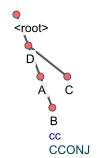
\includegraphics{img/nested1.png}
    \caption{Possible Wrong Attachments of a Coordinating Conjunction: Correct Head as Wrong Head's Sibling}
    \begin{flushleft}
    Note: \textit{D} is the common ancestor of nodes \textit{A}, \textit{B} and \textit{C}\\
    Note: \textit{C} is the more relevant head that conjunction \textit{B} should be attached to, instead of the current misdirected attachment with node \textit{A}\\
    Note: \textit{A}, \textit{C} and \textit{D} might be the head of their own subtrees
    \end{flushleft}
    \label{fig:conj-head1}
\end{figure}

\begin{figure}[H]
\begin{subfigure}{.45\textwidth}
  \centering
  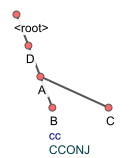
\includegraphics{img/nested2.png}
  \caption{Correct Head as Conjunction's Sibling}
  \label{fig:conj-head2}
  \end{subfigure}
\begin{subfigure}{.5\textwidth}
  \centering
  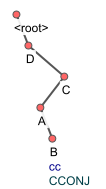
\includegraphics{img/nested3.png}
  \caption{Correct Head as Conjunction's Grandparent}
  \label{fig:conj-head3}
\end{subfigure}
\caption{Possible Wrong Attachments of a Coordinating Conjunction}
Note: \textit{D} is the common ancestor of nodes \textit{A}, \textit{B} and \textit{C}\\
Note: \textit{C} is the more relevant head that conjunction \textit{B} should be attached to, instead of the current misdirected attachment with node \textit{A}\\
Note: \textit{A}, \textit{C} and \textit{D} might be the head of their own subtrees
\label{fig:conj-head23}
\end{figure}

Notice that while the 3 cases as mentioned in Figures \ref{fig:conj-head1} and \ref{fig:conj-head23} are separate, there is no deterministic way of knowing what case an identified problematic instance might refer to. As such, we handle the 3 cases in decreasing order of priority, i.e. we try to handle the case as in Figure \ref{fig:conj-head1} first. In case the attempt fails, owing to multitude of reasons as explained later in Section \ref{ssec:conj_head_algorithm} (no siblings to attach to, lack of a candidate head in the siblings, for example), we try to solve it with respect to the case as in Figure \ref{fig:conj-head2}, and in case of a failure therein as well, eventually as in Figure \ref{fig:conj-head3}. If a particular instance is still not corrected after the consideration of the last case, we leave it unchanged.

\subsubsection{Conjunction Attached Non-Projectively}

In case of misdirected conjunctions that are attached non-projectively, the previous approach of limiting the level change with respect to the wrong head does not function well. The approach fails mainly because if the attachment is non-projective in nature, it is very likely that the conjunction is attached to a head in a different coordination. Consider the part of a sentence taken from UDv2.4 \verb|hi|-hdtb treebank in Example \ref{examp:conj_removed} and the tree for the corresponding example in Figure \ref{fig:conj_removed-wrong}. The token in bold is attached non-projectively because its current head is not a part of the same coordination structure as the conjunction itself.

\begin{example}
\label{examp:conj_removed}
\textbf{ }\\
\textbf{Text (\texttt{hi}):} \texthindi{वे सांसद \textbf{या} विधायक बनने के बाद लाभ के पद पर आसीन हैं या उससे पहले से हैं ।} \\
\textbf{Translit:} \textit{ve saamsad \textbf{yaa} vidhaayaka banane ke baada laabha ke pada para aasiin hain yaa usase pahale se hain .}\\
\textbf{Lit.:} they senator or legislator become-\textit{Inf.} \textit{Acc.} after power \textit{Poss.} position on situated are or therefrom before \textit{Dat.} are .\\
\textbf{Translated:} They have been in a position of power from before they became senator or legislator, or after.
\end{example}

\begin{figure}[H]
  \centering
  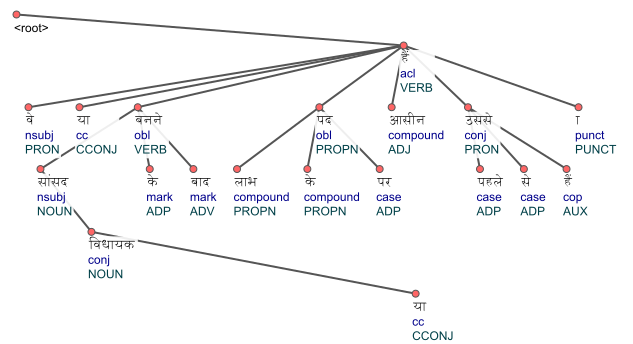
\includegraphics[scale=0.85]{img/removed-conj-wrong.png}
  \caption{Original Annotation for Example \ref{examp:conj_removed}}
  Note: First \texthindi{या} (\textit{yaa}, or) should be attached to \texthindi{विधायक} (\textit{vidhaayaka}; legislator), and not to \texthindi{हैं} (\textit{hain}; are)\\
  Note: Second \texthindi{या} (\textit{yaa}, or) should be attached to \texthindi{उससे} (\textit{usase}; therefrom), and not to \texthindi{विधायक} (\textit{vidhaayaka}; legislator)
  \label{fig:conj_removed-wrong}
\end{figure}

Since the conjunction is associated to a conjunct in the different coordination structure, the trivial approach to the problem is to look at the next available conjunct in the tree such that it satisfies the right-headedness criteria, and associate the conjunction to the said conjunct. In the previous example, the problem can simply be solved by associating the conjunction to the next available conjunct, marked by the deprel \verb|conj|. However, this might not be always possible if the next conjunct is not explicitly marked by the deprel. Consider the following example from UDv2.4 \verb|en|-EWT treebank and the associated dependency tree in Figure \ref{fig:nonconj}. The token of interest is marked in bold.

\begin{example}
\label{examp:nonconj}
\textbf{}\\
\textbf{But} other people do like the way they think he will vote, and the ones who favor him seem to outnumber the ones who oppose him .
\end{example}

\begin{figure}[H]
    \centering
    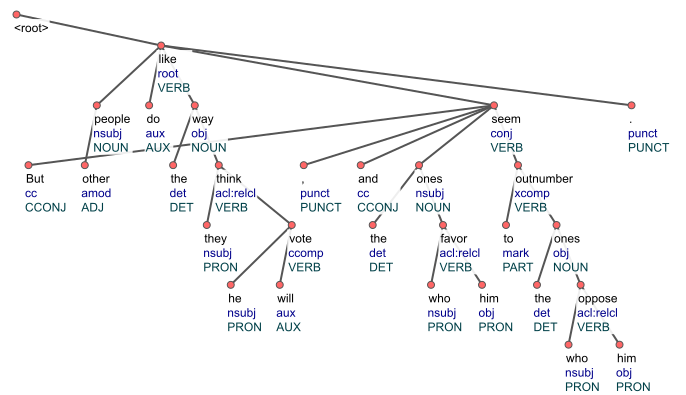
\includegraphics[scale=0.75]{img/nonconj.png}
    \caption{Dependency Tree for Example \ref{examp:nonconj}}
    Note: \textit{But} should be connected to \textit{like}, and not to \textit{seem}
    \label{fig:nonconj}
\end{figure}

In the example, the correct conjunct is not marked explicitly by the deprel \verb|conj|. Likewise in certain cases, the correct conjunct for the conjunction can not be found by the search for the deprel alone. However, based on the position of the content word token(s) that precede the conjunction in the word order, the correct conjunct can be determined to some extent. In the UDv2 guidelines, the dependencies that have a functional word as the head should be avoided (content-head dependency vs. function-head dependencies). Nonetheless, in some cases, the function words do form head of dependencies (when an auxiliary verb forms the root of a tree, for example). We treat the cases where the function word forms the head of a dependency as exceptional cases. As such, the correct conjunct position can be determined on the basis of the preceding content word token(s), including pronouns. The addition of pronouns is attributed to the fact that different pronouns can act as conjuncts in a sentence.

As can be seen in the last column in Tables \ref{tab:conjunctions_pud} and \ref{tab:conjunctions_all}, the misdirected dependencies such that they introduce non-projectivities are relatively uncommon. In our treatment of instances of the kind, we attempt to look for the next conjunct (if marked explicitly by the deprel) in the word order, such that the candidate conjunct follows the conjunction. In case the conjunct is not explicitly marked, we attempt to associate the conjunction to the immediately preceding content word in the word order. This ensures that the misdirection is not resolved, but the conjunction is now closer to the actual conjuncts and thus can be found in a process similar to the level-based analysis as done in previous subsection.

\subsection{Conjunction Sandwich}
\label{sec:conj-sand}

We have so far discussed only the cases where the problem can be identified by the wrong direction of dependency. However, when the direction of dependency is correct, mining for the problematic instances becomes troublesome. In Figure \ref{fig:conj_removed-wrong} reproduced below, notice that the first conjunction token \texthindi{या} (\textit{yaa}; or) is linked in the correct direction, but to the wrong head. This instance of the correct direction of attachment, albeit to wrong head, can be present in the original annotation, or might be introduced after the tree has been corrected for the misdirected dependency. We refer to such cases as a Conjunction Sandwich, since the conjunction is sandwich-ed in between the conjuncts, with a wrong choice of head but with the direction of attachment being as expected (right-headed in our case). The problem of not being able to identify the correct conjunct as elaborated earlier in Example \ref{examp:nonconj} can manifest itself in such cases as well, making this problem significantly harder to detect.

\begin{reusefigure}[H]{fig:conj_removed-wrong}
    \centering
    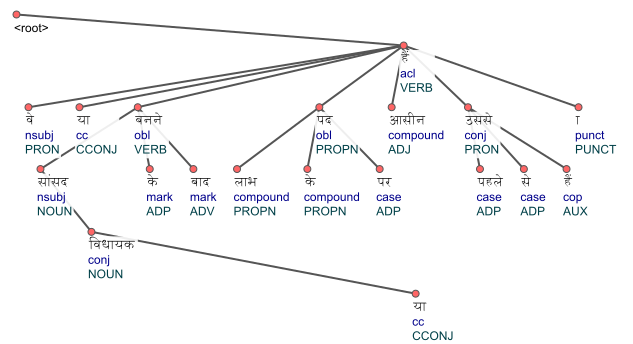
\includegraphics[scale=0.85]{img/removed-conj-wrong.png}
    \caption{Original Annotation for Example \ref{examp:conj_removed}}
    Note: First \texthindi{या} (\textit{yaa}; or) should be attached to \texthindi{विधायक} (\textit{vidhaayaka}; legislator), and not to \texthindi{हैं} (\textit{hain}; are)\\
  Note: Second \texthindi{या} (\textit{yaa}; or) should be attached to \texthindi{उससे} (\textit{usase}; therefrom), and not to \texthindi{विधायक} (\textit{vidhaayaka}; legislator)
\end{reusefigure}

In a given dependency tree, we can express node $A$ being followed by node $B$ in top-down ordering of tokens as $A < B$. To establish node $A$ is linked to node $B$, such that $A$ is the head of the relation, and $B$ is the dependent, we can write $A \rightarrow B$. In case where the direction of the relation is not important, we can express it by using double headed arrows as $A \leftrightarrow B$. 

In a dependency tree, given two undirected edges $i_{1} \leftrightarrow j_{1} \text{ and } i_{2} \leftrightarrow j_{2}$, the edges are said to be overlapping if $i_{1} < i_{2} < j_{1} < j_{2}$ or $i_{1} > i_{2} > j_{1} > j_{2}$. In the example figure above, we can see that one of the ways in which a case of conjunction sandwich manifests itself is in the form of overlapping edges. However, this might not always be the case. The edges can overlap also because of the faulty annotation of other tokens in the tree, and that renders this check unreliable. In the example figure above, the edge containing the first conjunction also overlaps with the edge containing second conjunction, attached non-projectively. The constraint (of overlapping edges) was also tightened to look for a conjunction being the sole node in the gap of a non-projective attachment, but the number of cases that were flagged in the process remained very low (mostly less than 1\% of total number of conjunctions across different languages, depending on the language as some languages allow less number of non-projective structures than others). Of the total number of cases that were flagged by the tighter constraint, the majority were false positives.

Consider the following example from UDv2.4 \verb|en|-lines treebank, and the associated dependency tree in Figure \ref{fig:unhandled-sandwich}. In this case, the edges do not overlap, but the conjunction is still attached to the wrong head.

\begin{example}
\label{examp:unhandled-sandwich}
\textbf{}\\
That was also mentioned by Mrs Oomen-Ruitjen \textbf{and} Mrs Glase.
\end{example}

\begin{figure}[H]
    \centering
    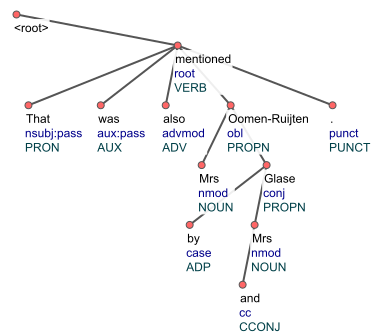
\includegraphics[scale=0.90]{img/unhandled-sandwich.png}
    \caption{Dependency Tree for Example \ref{examp:unhandled-sandwich}}
    Note: \textit{by} should be attached to \textit{Oomen-Ruitjen}, and not to \textit{Glase}\\
    Note: \textit{and} should be attached to \textit{Glase}, and not to \textit{Mrs}
    \label{fig:unhandled-sandwich}
\end{figure}

The trivial approach in the case of a Conjunction Sandwich would be to look for a conjunct explicitly marked by the \verb|conj| deprel, such that the said conjunct follows the conjunction in question. For example, in Figure \ref{fig:conj_removed-wrong}, the attachment for the first conjunction can be corrected by looking for the first explicitly marked conjunct that follows the current parent. This is an unreliable approach nonetheless, because (i) the conjunct needs to be explicitly marked by the deprel, which is not always the case; and (ii) the approach cannot work in the case of nested coordination, often picking up on a conjunct from another coordination structure.

Since none of the cases discussed in this section could be reliably scouted for, we do not deal with identification and/or correction of Conjunction Sandwich in the current research.

\section{Dataset}
\label{ssec:conj_head_dataset}

The experiment was initially started on UDv2.3 \citep{UDv2.3}, but owing to the release of UDv2.4 \citep{UDv2.4} in May 2019, the experiment was transported entirely to UDv2.4. It is worth noting that there were far more cases of this problem being identified in UDv2.3, rather than in UDv2.4. Nonetheless, there exist significant cases of the problem (attachment of a conjunction to an incorrect head, and in wrong direction) in UDv2.4 as well.

We limit our treatment of the problem to \verb|af|, and \verb|ar|. As can be seen from Table \ref{tab:conjunctions_all}, the languages contain treebanks such that (i) they do not display any postposed variant of conjunctions as denoted by asterisk superscript in the table; (ii) the number of misdirected dependencies in the treebank is more than 10\% of the total number of conjunctions; and (iii) the languages do not have non-projectivity as a major characteristic, and yet the number of misdirected non-projective attachments is high in the treebank (unlike \verb|grc| and \verb|la| which have non-projectivity as a characteristic feature). Additionally, the languages belong to different language families viz. Germanic Indo-European and Semitic Afro-Asiatic, thus ensuring that the results of the experiment are not specific to a limited set of languages.

The number of instances of misdirected dependencies in different treebanks of UDv2.4 was highlighted in Table \ref{tab:conjunctions_pud} and \ref{tab:conjunctions_all}. The count of instances for \verb|af|-afribooms and \verb|ar|-padt are highlighted again in Table \ref{tab:dataset_conj} for reference.

\begin{table}[H]
    \centering
    \begin{tabular}{|l|l|l|l|l|}
        \hline
        \textbf{Treebank} & \textbf{Total} & \textbf{Misdirected} & \textbf{\% Total} & \textbf{Non-Proj}\\
        \hline
        \verb|af|-afribooms & 1 832 & 1 829 & 99.836 & 130\\
        \verb|ar|-padt & 13 855 & 1 411 & 10.184 & 80\\
        \hline
    \end{tabular}
    \caption{Misdirected Coordinating Conjunctions in UDv2.4 Treebanks for \texttt{af} and \texttt{ar}}
    \label{tab:dataset_conj}
\end{table}

\section{Experimental Setup}
\label{ssec:conj_head_experiment}

At the end of Section \ref{sec:conj-sand}, we mentioned how we would not deal with the cases where the direction of attachment is already correct. Thus, in the experiments, our treatment is limited to the instances with misdirected dependencies. To that resort, we start by identification of conjunctions such that they are associated in the wrong direction. Upon identification of such tokens, if they are attached non-projectively, we associate the token (still in the wrong direction) to the nearest content word that precedes the said token. In case the new attachment is now projective, we can terminate dealing with this case here. In the case of the new attachment being non-projective again, we try finding a content word (including pronouns) that is closest to the conjunction in word-order, and try attachment with this found word. If the new attachment is projective, we have dealt with the problem of non-projectivity for now, and the node in question can be associated to a more relevant head as other nodes that were originally projectively attached.

The problem with this approach (of reducing a case of non-projective attachment artificially to that of a projective attachment) is twofold. Primarily, the algorithm, as mentioned in Section \ref{ssec:conjunct-search}, looks for the candidate conjunct at a level that is determined by the attachment to the wrong conjunct. In principle, the choice of a wrong parent while solving non-projectivity could eventually lead to the corrected attachment with the wrong parent, resulting in a conjunction sandwich. Secondly, the approach does not take into account the cases when the attachment needs to be made to a function word, rather than a content word. The same issue can be raised for even the way the projective attachments are handled in general.

\section{Algorithm}
\label{ssec:conj_head_algorithm}

We start with defining some wrapper functions in Algorithm \ref{misdirected-edges-algo} and \ref{rollback-algo}. While the first one checks for the coordinating conjunctions that are attached in wrong direction, the second one tries to change the parent of the given node $x$ to a new parent $z$. In case the new attachment would be non-projective, the function rolls back to the previous parent. If projectivity is preserved, the function returns a \textbf{true} value, which allows us to terminate the function whenever the function call is made inside another function. The function also checks against making the node attached directly to the root of the tree, thereby making sure there is just one root node at any instance.

\begin{algorithm}[H]
\caption{misdirectedDependency()}
\label{misdirected-edges-algo}
    \begin{algorithmic}[1]
    \REQUIRE Node $x$
    \IF {$x.upos$ == ``CCONJ" \AND $x.udeprel$ == ``cc" \AND $x.parent.id$ < $x.id$}
        \RETURN \TRUE
    \ENDIF
    \RETURN \FALSE
    \end{algorithmic}
\end{algorithm}

\begin{algorithm}[H]
\caption{setParent()}
\label{rollback-algo}
    \begin{algorithmic}[1]
    \REQUIRE Node $x$, Original Parent $y$, New Parent Candidate $z$
    \STATE $x.parent \leftarrow z$
    \IF {$isnonprojective(x) == \TRUE$ \OR $z.id == 0$}
        \STATE $x.parent \leftarrow y$
        \RETURN \FALSE
    \ELSE
        \RETURN \TRUE
    \ENDIF
    \end{algorithmic}
\end{algorithm}

Having defined our wrapper functions, we start by trying to projectivize the conjunctions attached non-projectively in the wrong direction. We start by first looking for the next explicitly marked conjunct, and try to attach the conjunction to the said conjunct. We define this procedure in Algorithm \ref{algo:search-content}.

\begin{algorithm}[H]
\caption{nextConjHead()}
\label{algo:search-content}
    \begin{algorithmic}[1]
    \REQUIRE Node $x$ such that  $misdirectedDependency(x) == \TRUE$ \AND $isnonprojective(x) == \TRUE$, Original Parent $y$
    \STATE List $L \leftarrow$ containing nodes arranged in the increasing order of their $id$
    \STATE \COMMENT{i.e. $i < j \implies L[i].id < L[j].id \hspace{5mm} \forall L[i], L[j] \in L$}
    \FOR{node $z$ in $L$}
    \STATE \COMMENT{Process nodes in increasing order of their $id$}
        \IF {$z.id$ > $x.id$}
            \IF {$z.udeprel == ``conj"$}
                \RETURN $setParent(x, y, z)$
            \ENDIF
        \ENDIF
    \ENDFOR
    \RETURN \FALSE
    \end{algorithmic}
\end{algorithm}

In case of scenarios like in Example \ref{examp:conj_removed} (figure reproduced again below) with respect to the second conjunction, the non-projective attachment is made projective, and rectified with respect to the correct head automatically. However, there are cases when this approach may fail, owing to the next marked conjunct being located far away (and thus new attachment being non-projective again) or the next conjunct not being marked explicitly. In such cases, we move to the next step, and try to associate the current conjunction to the content word or pronoun that immediately precedes the given token. To look for the immediately preceding content word or pronoun, we look for the following POS tags- \verb|ADJ|, \verb|ADV|, \verb|NOUN|, \verb|PROPN|, \verb|VERB|, and \verb|PRON|. As with previous approach, we rollback the changes in case the attachment to new candidate head is non-projective in nature, going back to the original parent. The procedure is elaborated in Algorithm \ref{algo:conj-head-nonproj}.

\begin{reusefigure}[H]{fig:conj_removed-wrong}
    \centering
    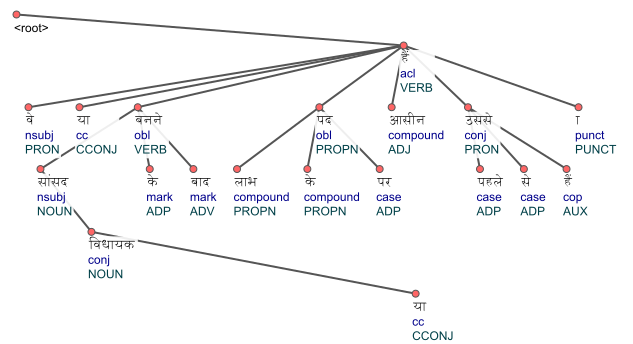
\includegraphics[scale=0.85]{img/removed-conj-wrong.png}
    \caption{Original Annotation for Example \ref{examp:conj_removed}}
    Note: First \texthindi{या} (\textit{yaa}; or) should be attached to \texthindi{विधायक} (\textit{vidhaayaka}; legislator), and not to \texthindi{हैं} (\textit{hain}; are)\\
  Note: Second \texthindi{या} (\textit{yaa}; or) should be attached to \texthindi{उससे} (\textit{usase}; therefrom), and not to \texthindi{विधायक} (\textit{vidhaayaka}; legislator)
\end{reusefigure}


\begin{algorithm}[H]
\caption{projTempFix()}
\label{algo:conj-head-nonproj}
\begin{algorithmic}[1]
\REQUIRE Node $x$ such that $misdirectedDependency(x) == \TRUE$ \AND $isnonprojective(x) == \TRUE$, Original Parent $y$
\STATE $candidates$ = []
\STATE \COMMENT{Empty List}
\FORALL{$z$ such that $z.id$ < $x.id$}
    \IF{$z.upos$ in $[``ADJ", ``ADV", ``NOUN", ``PROPN", ``VERB", ``PRON"]$}
        \STATE $candidates.append(z)$
        \STATE \COMMENT{Add $z$ to $candidates$ list}
    \ENDIF
\ENDFOR
\STATE \COMMENT{The content nodes are organised in the list, in word-order. We need to work with only the last candidate.}
\IF{$candidates$ == []}
    \RETURN \FALSE
\ELSE
    \STATE $candidate$ = $candidates[-1]$
    \STATE \COMMENT{Pick up the last element from $candidates$ list, and try changing it to head}
    \RETURN $setParent(x, y, candidate)$
\ENDIF
\end{algorithmic}
\end{algorithm}

Using the above algorithm, we are able to find better candidates for the originally misdirected non-projective dependency. Consider the following sentence, as taken from UDv2.4 \verb|af| treebank in Example \ref{examp:projTempFix}, and the corresponding original and modified annotations in Figure \ref{fig:projTempFixexample}, with the token of interest marked in bold. We can see that the original annotation contains the conjunction attached non-projectively. However, following the correction, the non-projectivity is solved and the new attachment is closer to the correct annotation. It is worth noting that the non-projectivity related to the punctuation marks can be solved easily (cf. Section \ref{ssec:punct-nonproj}).

\begin{example}
\label{examp:projTempFix}
\textbf{ }\\
\textbf{Text (\texttt{af}):} Ons onderwysteikens is eenvoudig , \textbf{maar} van kritiese belang.\\
\textbf{Lit:} Our educational-target\textit{-Pl.} is simple , \textbf{but} of critical significance .\\
\textbf{Translated:} Our educational targets are simple, but of critical significance.
\end{example}
\begin{figure}[H]
    \centering
    \begin{subfigure}{\textwidth}
    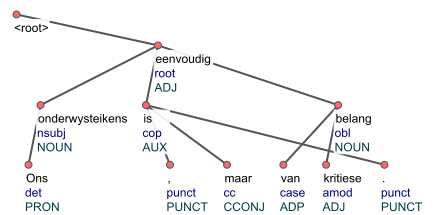
\includegraphics{img/projTempFixOriginal.png}
    \caption{Original Annotation}
    \end{subfigure}
    \begin{subfigure}{\textwidth}
    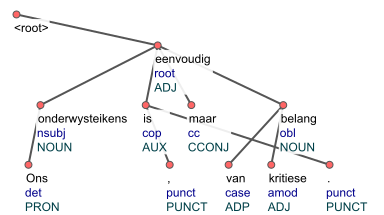
\includegraphics{img/projTempFixModified.png}
    \caption{Modified Annotation}  
    \end{subfigure}
    \caption{Change in Annotation for Example \ref{examp:projTempFix}}
    Note: \textbf{maar} (but) should be attached to \textbf{belang} (significance)
    \label{fig:projTempFixexample}
\end{figure}

At this point, we have exhausted our treatment of non-projective misdirected dependencies. A misdirected non-projective attachment of conjunction is either projective after this step, or is unaffected. We discuss the second case in Section \ref{ssec:conj_head-results} when we discuss the results of the experiment in more detail. For the first case of non-projective attachments, we have now removed the non-projectivity from the attachment, making sure they can be handled in the same manner as the other originally projective attachments, as elaborated earlier. 
% shown in Figures \ref{flow:conj_head_nonproj} and \ref{flow:conj_head_proj}.

For the common treatment of the attachments independent of their projectivity status, we look for the conjunctions such that they are attached in wrong direction. As a first step in search for a candidate conjunct, we look for the content words at the same level as the current node. We start by checking if there is a single remaining sibling that does not have a POS tag of \verb|X|, \verb|PUNCT|, or \verb|SYM| since we want to avoid the linking of the conjunction to these POS tags. In case of the condition being satisfied, and thus the availability of a single sibling as a candidate head, the token of interest is tried to be attached to this candidate head, and a \textbf{true} value is returned, indicating the success in search for the candidate. The effectiveness of case when a single sibling is present is demonstrated in Figure \ref{fig:singleSiblingAttach} containing an extension of the Example \ref{examp:projTempFix}, after the modification from Figure \ref{fig:projTempFixexample}.

\begin{figure}[H]
    \centering
    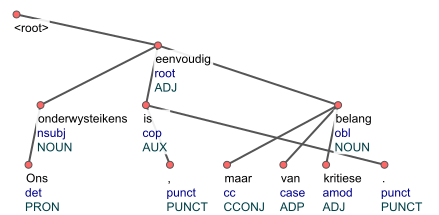
\includegraphics{img/projTempFixFinal}
    \caption{\textit{attachToSibling()}: Single Sibling Available}
    \label{fig:singleSiblingAttach}
\end{figure}

In case there are multiple siblings, we try to find the nearest sibling that has the deprel as \verb|conj|, and try attaching the conjunction to this marked conjunct. Essentially, this check would ensure that there is no need to search for another candidate, as the nearest sibling is the one that should be the head. In case the attachment to the marked conjunct will be non-projective in nature, the candidate would be located further away, and is not fit to being the head. However, this approach might fail owing to the conjunct not being explicitly marked. In the final search for the candidate conjunct in the siblings, we try to find the candidate by restricting the deprels to \verb|obl|, \verb|xcomp|, \verb|nmod|, and \verb|nsubj| amongst the siblings, attaching therein if such a case is found. 

The choice of the deprels is not arbitrary, but is based on an elimination procedure whereby we discarded most deprels. For selection of the candidate deprels, we restricted ourself to the core arguments, non-core dependents and nominal dependents that correspond to nominal and clausal structural categories\footnote{The first two columns, and the entries against the structural categories as indicated in \url{https://universaldependencies.org/u/dep/all.html}}. Of these relations, \verb|dislocated|, \verb|expl|, \verb|nummod|, \verb|vocative| can be outright discarded from the consideration. For \verb|appos|, the documentations marks explicitly the case where the deprel is chained in presence of a coordination\footnote{\url{https://universaldependencies.org/u/dep/appos.html}}, marking the subsequent tokens as \verb|conj|, rather than as \verb|appos|. The deprels \verb|acl| and \verb|advcl| function as clausal modifiers in form of an adjective\footnote{\url{https://universaldependencies.org/u/dep/acl.html}}, or an adverb\footnote{\url{https://universaldependencies.org/u/dep/advcl.html}} respectively. Since the dependents are explicitly clausal, we can very well discard them from consideration of conjuncts, alongwith \verb|appos|.

The documentations for the deprels \verb|obj|\footnote{\url{https://universaldependencies.org/u/dep/obj.html}} and \verb|iobj|\footnote{\url{https://universaldependencies.org/u/dep/iobj.html}} states that in presence of more than one proto-patients, the primary is to be labelled as \verb|obj|, and the rest as \verb|iobj|. However, even in presence of multiple objects (tri-transitive verbs are rare, but nonetheless present in Caucasian languages like Georgian, and Svan for example), the objects to the verb are often associated in form of causatives (cf. \cite[p.~39]{chirikba}, \cite[p.~43]{boeder}). This can be further extrapolated into a lack of conjunction between such objects of the tri-transitive verbs, thereby ensuring that we can safely discard the deprels \verb|obj| and \verb|iobj| from our consideration as well. 

The documentation\footnote{\url{https://universaldependencies.org/u/dep/csubj.html}} for deprel \texttt{csubj} states that the deprel is used when the subject itself is a clause. The guideline would ensure that there are very few cases when the deprels might be chained together by coordination, and even more so while they are at the same level in the tree. We therefore remove the deprel from consideration. 

Comparing the documentations of \texttt{ccomp}\footnote{\url{https://universaldependencies.org/u/dep/ccomp.html}} and \texttt{xcomp}\footnote{\url{https://universaldependencies.org/u/dep/xcomp.html}}, there is no way to say if either deprel is a better fit for the candidate head. In our experiments, the experiment performance went down when \texttt{ccomp} was included in the final list of head deprels. Keeping that in mind, we only include \texttt{xcomp} and discard \texttt{ccomp} from our consideration of candidate head deprels.

We could not find a strong reason for discarding the remaining deprels, viz. \verb|obl|, \verb|nmod|, and \verb|nsubj|, and thus included them with \verb|xcomp| in the list of deprels that can be searched for, while looking for a candidate conjunct.

The restriction with respect to deprels is necessary to make sure we don't over-generate and rehang the conjunction to a wrong head. As demonstrated earlier, a non-first conjunct may or may not be labelled by the \texttt{conj} deprel. The deprels associated with the core arguments, non-core dependents and nominal dependents are governed (non-deterministically) by the POS tag of a token and the head of this token, whereas the \texttt{conj} deprel is not limited by the POS tag of either the token or its head. Therefore, we can rely upon the other deprels to be annotated better than the \texttt{conj} relation. However, if the deprel is not restricted, the token of interest might associate itself to the wrong sibling, but in the correct direction, making it as a case of a conjunction sandwich (which as we mentioned earlier, is significantly harder to detect).

We formally define the constraints and the processing in Algorithm \ref{conj-head-sibling}. Notice how we decide on whether or not the algorithm terminates by continuously checking the condition of projectivity, and returning a value from the function only if the condition of projectivity with respect to the new parent is maintained. It is also important to note that we always limit our search for a suitable candidate to cases where the candidate occurs later than the conjunction we are trying to rehang.

\begin{algorithm}[H]
\caption{attachToSibling()}
\label{conj-head-sibling}
\begin{algorithmic}[1]
\REQUIRE $node$ such that $misdirectedDependency(node) == \TRUE$
\STATE \COMMENT{Try to attach to a sibling node}
\STATE $count \leftarrow 0$
\STATE $origParent \leftarrow node.parent$
    \FORALL {$siblings$ of $node$} \label{line:conj-sibling-countcheck1}
        \IF {$siblings.upos$ not in $[``X", ``PUNCT", ``SYM"]$ \AND $siblings.id > node.id$}
            \STATE $TargetSibling \leftarrow siblings$
            \STATE $count \leftarrow count + 1$
        \ENDIF
    \ENDFOR
    \IF {$count == 1$}
        \STATE \COMMENT{Just one sibling, attach to this sibling}
        \IF {$setParent(node, origParent, TargetSibling)$}
            \RETURN \TRUE
        \ENDIF
    \ENDIF \label{line:conj-sibling-countcheck2}
    \STATE \COMMENT{More than one siblings, narrow search by deprels}
    \FOR {$sibling$ of $node$}
        \IF {$sibling.udeprel == ``conj"$ \AND $sibling.id > node.id$}
            \IF {$setParent(node, origParent, sibling)$}
                \RETURN \TRUE
            \ENDIF
        \ENDIF
    \ENDFOR
    \FOR {$sibling$ of $node$}
        \IF {$sibling.udeprel$ in $[``obl", ``xcomp", ``nmod", ``nsubj"]$ \AND $node.id < sibling.id$}
            \IF {$setParent(node, origParent, sibling)$}
                \RETURN \TRUE
            \ENDIF
        \ENDIF
    \ENDFOR
\RETURN \FALSE
\end{algorithmic}
\end{algorithm}

If there is no suitable candidate in the same level as the current level of the conjunction, we try to ascend one level and try to attach the node to the next aunt (parent's sibling) in Algorithm \ref{conj-head-aunt}. The condition may arise owing to not finding a suitable candidate in siblings, or in case where there are no siblings to search for. We do not set any checks with respect to deprels, but still keep a check on the condition of projectivity and the node order. Consider the following part of sentence from \verb|af| treebank in Example \ref{examp:auntAttach} with the corresponding annotations in Figure \ref{fig:auntAttach}, with the token of interest marked in bold. Figure \ref{fig:auntAttach-2} shows the part where the algorithm connects the conjunction to the parent's sibling, after having failed trying to find an attachment amongst the siblings.

\begin{algorithm}[H]
\caption{attachToAunt()}
\label{conj-head-aunt}
\begin{algorithmic}[1]
\REQUIRE $node$ such that $misdirectedDependency(node) == \TRUE$
\STATE \COMMENT{Try to attach to the first relevant aunt node}
\STATE $origParent \leftarrow node.parent$
\STATE $aunts = []$
\FOR {$sibling$ of $origParent$}
    \IF {$sibling.id > node.id$}
        \STATE $aunts$.append($sibling$)
    \ENDIF
\ENDFOR
\STATE \COMMENT{The candidate aunts would be arranged in word-order in the $aunts$ list}
\IF {$aunts$ is not empty}
    \STATE $setParent(node, origParent, aunts[0])$
\ENDIF
\RETURN \FALSE
\end{algorithmic}
\end{algorithm}

\begin{example}
\label{examp:auntAttach}
\textbf{ }\\
\textbf{Text (\texttt{af}):} Indien die laaste dag vir betaling op 'n openbare vakansiedag \textbf{of} oor die naweek val, ... \\
\textbf{Lit:} In-the-event-that the last day for pay on a public holiday \textbf{or} over the weekend fall, ...\\
\textbf{Translated:} If the last day for payment falls on a public holiday or over the weekend, ...
\end{example}

\begin{figure}
    \centering
    \begin{subfigure}{\textwidth}
    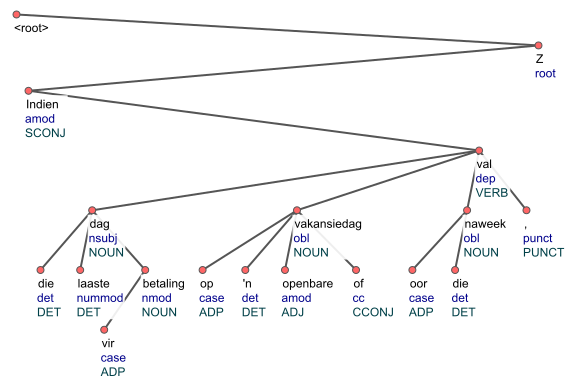
\includegraphics[scale=0.80]{img/auntAttachOriginal.png}
    \caption{Original Annotation}
    \label{fig:auntAttach-1}
    \end{subfigure}
    \begin{subfigure}{\textwidth}
    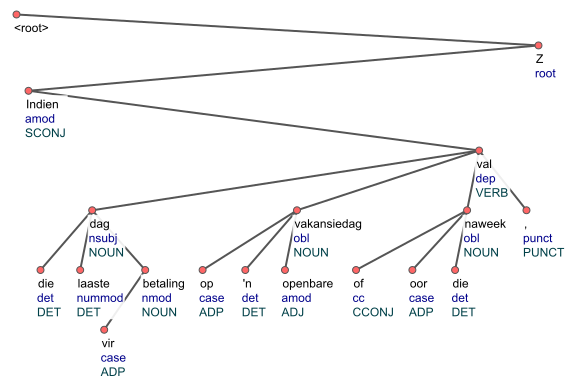
\includegraphics[scale=0.80]{img/auntAttachFinal.png}
    \caption{Modified Annotation after attachToAunt()}
    \label{fig:auntAttach-2}
    \end{subfigure}
    \caption{Change in Annotation for Example \ref{examp:auntAttach}}
    Note: \textit{Z} is used to denote the position of original root of the sentence\\
    Note: \textbf{of} (or) should be attached to \textbf{naweek} (weekend)
    \label{fig:auntAttach}
\end{figure}

In the event that a suitable candidate is not found, a \textbf{false} value is returned. This implies that our search for a suitable candidate has failed even after trying to ascend one level. As last resort, we try to attach the conjunction to the grandparent, while preserving projectivity in Algorithm \ref{conj-head-granny}. An example of case where this function is needed is elaborated in Example \ref{examp:granny} containing the sentence from \verb|af| treebank, with the corresponding annotations in Figure \ref{fig:granny}.

\begin{algorithm}[H]
\caption{attachToGrandparent()}
\label{conj-head-granny}
\begin{algorithmic}[1]
\REQUIRE $node$ such that $misdirectedDependency(node) == \TRUE$
\STATE \COMMENT{Try to attach to the grandparent node}
\STATE $origParent \leftarrow node.parent$
\STATE $grandparent \leftarrow origParent.parent$
\IF {$setParent(node, origParent, grandparent)$}
    \RETURN \TRUE
\ENDIF
\RETURN \FALSE
\end{algorithmic}
\end{algorithm}

\begin{example}
\label{examp:granny}
\textbf{ }\\
\textbf{Text (\texttt{af}):} Ons onderwys- \textbf{en} vaardigheidsprogramme sal ons produktiwiteit en mededingendheid verhoog . \\
\textbf{Lit:} Our education- \textbf{and} skills-program-\textit{Pl.} shall our productivity and competitiveness increase .\\
\textbf{Translated:} Our education and skills programs will increase our productivity and competitiveness.
\end{example}

\begin{figure}[H]
    \centering
    \begin{subfigure}{\textwidth}
    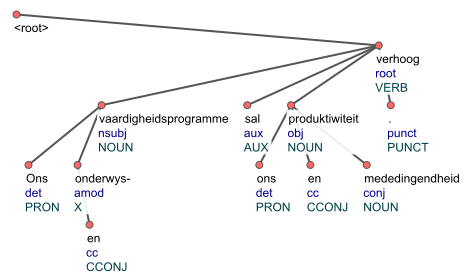
\includegraphics[scale=0.80]{img/grannyOriginal.png}
    \caption{Original Annotation}
    \label{fig:granny-1}
    \end{subfigure}
    \begin{subfigure}{\textwidth}
    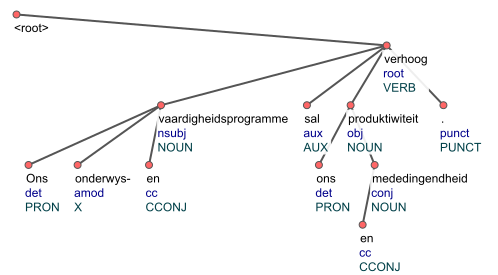
\includegraphics[scale=0.80]{img/grannyModified.png}
    \caption{Modified Annotation after attachToGrandparent()}
    \label{fig:granny-2}
    \end{subfigure}
    \caption{Change in Annotation for Example \ref{examp:granny}}
    Note: \textbf{en} (and) should be attached to \textbf{vaardigheidsprogramme} (skills-program)
    \label{fig:granny}
\end{figure}

Having established all the possible cases, we can wrap them all in a nice function that takes care of all the cases, in priority order. Algorithm \ref{conj-head-algo} shows the complete algorithm, in order of execution of the functions defined throughout the section.

\begin{algorithm}[H]
\caption{fixconjhead()}
\label{conj-head-algo}
\begin{algorithmic}[1]
\REQUIRE $node$ such that $misdirectedDependency(node) == \TRUE$
\IF{$isnonprojective(node)$ == \TRUE}
    \IF{\NOT{$nextConjHead(node, node.parent)$}}
        \IF{\NOT{$projTempFix(node, node.parent)$}}
            \STATE Do Nothing
        \ENDIF
    \ENDIF
\ENDIF
\STATE \COMMENT{Made non-projective attachments projective}
\IF {$attachToSibling(node)$}
    \RETURN 
\ELSIF{$attachToAunt(node)$}
    \RETURN
\ELSIF{$attachToGrandparent(node)$}
    \RETURN
\ELSE
    \RETURN
\ENDIF
\end{algorithmic}
\end{algorithm}

\section{Evaluation and Results}
\label{ssec:conj_head-results}

We implement the algorithm in form of a Udapi-python \citep{udapi} block\footnote{Code alongwith manually annotated data available at \url{https://github.com/Akshayanti/Masters-Thesis-CUNI-2020/tree/master/conj_head}}. The runtime of the block for the data is as mentioned in Table \ref{tab:conj-head-runtime}, as run on Ubuntu 18.04 (64-bit) on a 4-core Intel i5-6300 HQ processor.

\begin{table}[H]
    \centering
    \begin{tabular}{|l|l|}
        \hline
        \textbf{Language} & \textbf{Time (in ms)}\\
        \hline
        \verb|af| & $81.33 \pm 7.094$ \\
        \verb|ar| & $317.05 \pm 23.996$ \\
        \hline
    \end{tabular}
    \caption{Average Runtime ($\pm$ sd) for Udapy Python Block Implementation}
    Note: Does Not include time taken to read the original CoNLL-U file
    \label{tab:conj-head-runtime}
\end{table}

In this section, we would first evaluate the treatment of originally nonprojective attachments with respect to the individual segments of the algorithm, followed by a discussion of the instances not handled by the algorithm dealing specifically with nonprojective attachments. The instances were manually annotated for the direction of dependency, as well as for the choice of the correct head. Next, we would look at the part of the algorithm that is common to all tokens, irrespective of their projectivity status. Our focus would be on the nodes that were affected at major steps, and the nodes that were unaffected by the end of the algorithm. We then look at the overall evaluation of the algorithm, as manually annotated for the correct attachment to the parent node, on limited subsamples.

\subsection{Originally Non-Projective Attachments}

The number of originally nonprojective nodes affected by the first part of the algorithm, where they were associated with either the next marked conjunct, or where their attachment was temporarily made projective is as listed in Table \ref{tab:affectedNodes1}. We discuss on the effect of individual functions in the following subsections.

\begin{table}[H]
\centering
    \begin{tabular}{|l|l|l|l|l|}
        \hline
        \textbf{Lang.} & \textbf{Total} & \textit{nextConjHead()} & \textit{projTempFix()} & Unaffected\\
        \hline
        \texttt{af} & 130 & 20 & 106 & 5\\
        \texttt{ar} & 80 & - & 44 & 36\\
        \hline
    \end{tabular}
    \caption{Nodes Affected: Non Projective Attachment}
    \label{tab:affectedNodes1}
\end{table}

\subsubsection{Effect of \textit{nextConjHead()}}

Of all the nodes affected by \textit{nextConjHead()} algorithm (cf. Algorithm \ref{algo:search-content}), 85\% of the nodes were associated to the right parent. Of the remaining 15\%, we found annotation errors which resulted in a failure in identification of the more relevant head. The annotation errors in these case were primarily associated with the wrong token being marked as a conjunct, or an explicitly marked conjunct of another coordination structure being selected as candidate (the conjunct in current coordination structure was not explicitly marked). While the modified annotation in these cases corrected the direction of dependency, there was a failure in determination of the correct head of attachment. This is a case of conjunction sandwich, as discussed earlier, and introduced in this context owing to a faulty correction. An example of such case is shown in Example \ref{examp:nextConjHead-wrong}, with the associated annotations in Figure \ref{fig:nextConjHead-wrong}. As before, the token of interest is marked in bold.

\begin{example}
\label{examp:nextConjHead-wrong}
\textbf{ }\\
\textbf{Text (\texttt{af}):} ... in hulle huise, op straat \textbf{en} op die pad in voortdurende angs verkeer ...\\
\textbf{Lit:} ... in \textit{3Pl-Poss.} house, on street \textbf{and} on the path-\textit{Sg.} in continuous anxiety find-\textit{Pres.} ...\\
\textbf{Translated:} ... in their house, on street and on the road in continuous anxiety ...
\end{example}

\begin{figure}[H]
    \begin{subfigure}{.49\textwidth}
     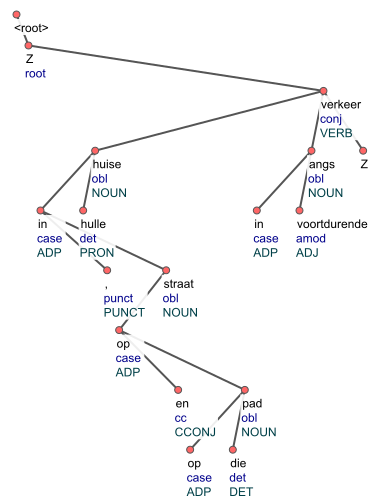
\includegraphics[scale=0.69]{img/nextConjHead-wrong1.png}
     \caption{Original Annotation}
    \end{subfigure}
    \begin{subfigure}{.5\textwidth}
    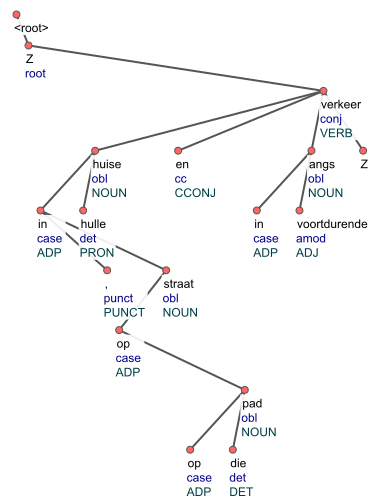
\includegraphics[scale=0.69]{img/nextConjHead-wrong2.png}
     \caption{Final Annotation}
    \end{subfigure}
    \caption{Annotation Error in Example \ref{examp:nextConjHead-wrong}}
    Note: Z is used as a placeholder for omitted text\\
    Note: \textbf{,} should be attached to \textbf{huise} (house) or to the immediately succeeding \textbf{op} (on)\\
    Note: \textbf{straat} (street) and its children should be attached to \textbf{verkeer} (find-\textit{Pres.})\\
    Note: \textbf{en} (and) should be attached to \textbf{pad} (path-\textit{Sg.}) \\
    Note: \textbf{pad} (path-\textit{Sg.}) and its children should be attached to \textbf{verkeer} (find-\textit{Pres.})\\
    Note: \textbf{verkeer} (find-\textit{Pres.}) is wrongly marked as \verb|conj|
    \label{fig:nextConjHead-wrong}
\end{figure}

\subsubsection{Effect of \textit{projTempFix()}}

Table \ref{tab:projTempFixResults} shows the number of instances that were forced into a projective attachment when \textit{projTempFix()} algorithm (cf. Algorithm \ref{algo:conj-head-nonproj}) was used on them. The total count of such instances is listed in the second column. The values in third column onward refer to the results of the manual verification, verified with respect to the direction of new attachment and the relevancy of the choice of head for the new attachment. The manual verification was done after the projectivised token was subjected to the overall algorithm. The third column refers specifically to the cases where the direction was corrected, but the choice of head of attachment was not correct, thereby resulting in a conjunction sandwich. The value in the fourth column refers to the count of tokens that had no change whatsoever in their attachment, before and after the algorithm. The value in the last column represents the count of tokens such that the attachment to new parent was correct in both the aspects.

\begin{table}[H]
    \centering
    \begin{tabular}{|l|l|l|l|l|}
    \hline
    \textbf{Lang.} & \textbf{Total} & Conj. Sand. & Unfixed & Correct\\
    \hline
    \texttt{af} & 106 & 12 & 91 & 3\\
    \texttt{ar} & 44 & - & 42 & 2\\
    \hline
    \end{tabular}
    \caption{Evaluation: \textit{projTempFix()}}
    \label{tab:projTempFixResults}
\end{table}

While the results for the forced projectivisation are primarily negative, there seems to be a pattern to the results. In the analysis of the instances marked as unfixed for either language, it was found that the correct attachment was not possible because the relevant part of the dependency tree had the original annotation wrong and non-projective while the correct annotation would be projective. Consider one such instance in Example \ref{examp:projTemp00}, and the associated dependency trees in Figure \ref{fig:projTemp00}, with the token of interest marked in bold. Notice the adposition \textbf{van} (of) being shared wrongly with \textbf{kultuur} (culture) token in Figures \ref{projTempFix00-orig}, \ref{projTempFix00-mod}. The overall corrected annotation is reflected in Figure \ref{projTempFix00-correct1}.

\begin{example}
\label{examp:projTemp00}
\textbf{ }\\
\textbf{Text (\texttt{af}):} ``deure van geleerdheid \textbf{en} van kultuur"\\
\textbf{Lit:} `` doors of learning \textbf{and} of culture " \\
\textbf{Translated:} ``doors of learning and of culture"
\end{example}

\begin{figure}[H]
    \begin{subfigure}{.45\textwidth}
    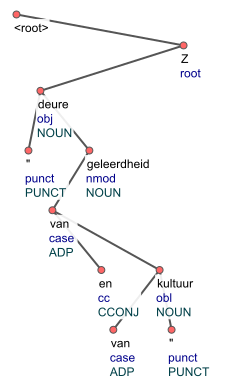
\includegraphics[scale=0.80]{img/projTempFix00-orig.png}
    \caption{Original Annotation}
    \label{projTempFix00-orig}  
    \end{subfigure}
    \begin{subfigure}{.5\textwidth}
    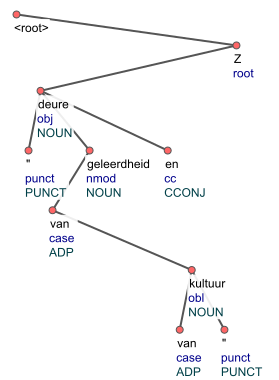
\includegraphics[scale=0.80]{img/projTempFix00-mod.png}
    \caption{Final Annotation}
    \label{projTempFix00-mod}  
    \end{subfigure}
    \begin{subfigure}{\textwidth}
    \centering
    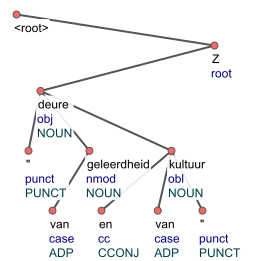
\includegraphics[scale=0.80]{img/projTempFix00-correct1.png}
    \caption{Overall Corrected Annotation}
    \label{projTempFix00-correct1}  
    \end{subfigure}
    \caption{Dependency Trees for Example \ref{examp:projTemp00}}
    Note: \textit{Z} is used to denote the node where the subtree is attached in the original sentence
    \label{fig:projTemp00}
\end{figure}

The problem of the false annotations with respect to non-projectivity is an open problem that is not handled in the current work. The problem is discussed in brief in Section \ref{future:nonproj}. In the current context, the cases of conjunction sandwich are also attributed to such wrong annotations. Consider the sentence from \verb|af| treebank in Example \ref{examp:projTemp01} and the associated dependency trees in Figure \ref{fig:projTemp01}, with the token of interest marked in bold. Note that the adposition \textbf{vir} (for) is shared wrongly by \textbf{besending} (consignment), bringing false non-projectivity into the sentence structure. 

\begin{example}
\label{examp:projTemp01}
\textbf{ }\\
\textbf{Text (\texttt{af}):} Hierdie permit is vir 'n beperkte tydperk \textbf{en} vir slegs een besending geldig .\\
\textbf{Lit:} this permit is for a limited period \textbf{and} for only one consignment valid . \\
\textbf{Translated:} This permit is valid for a limited period and for only one consignment.
\end{example}

\begin{figure}[H]
    \begin{subfigure}{\textwidth}
    \centering
    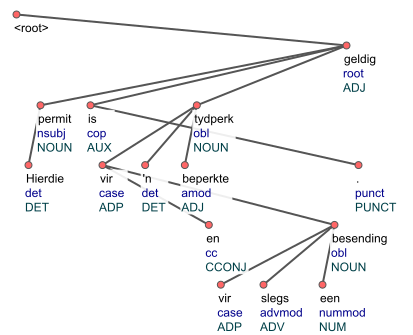
\includegraphics[scale=0.80]{img/projTempFix01-orig.png}
    \caption{Original Annotation}
    \label{projTempFix01-orig}  
    \end{subfigure}
    \begin{subfigure}{\textwidth}
    \centering
    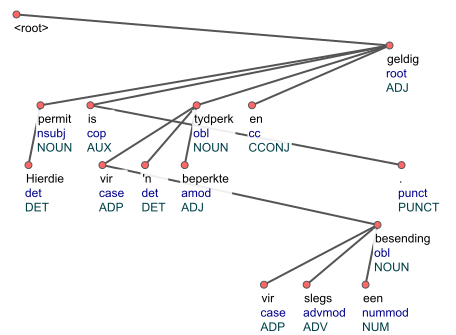
\includegraphics[scale=0.80]{img/projTempFix01-mod.png}
    \caption{Final Annotation}
    \label{projTempFix01-mod}  
    \end{subfigure}
    \caption{Dependency Trees for Example \ref{examp:projTemp01}}
    Note: \textbf{besending} (consignment) should be linked to \textbf{geldig} (valid)\\
    Note: \textbf{en} (and) should be linked to \textbf{besending} (consignment)\\
    Note: \textbf{.} should be linked to \textbf{geldig} (valid)
    \label{fig:projTemp01}
\end{figure}


\subsubsection{Non-Projective Attachments Not Handled}

All the cases that were unprocessed after the attempt at projectivisation of non-projective attachments were processed by the overall algorithm. We do not discuss here the statistics on the correction procedure of such cases, but leave it for the next section when we evaluate the overall algorithm. 

\subsection{Processing Pipeline Independent of Projectivity of Attachment}

As can be seen from Table \ref{tab:affectedNodesOverall}, the manual evaluation if done on a randomly chosen sample of the affected nodes would be very heavily biased on the results from \textit{attachToSibling()} algorithm. To counter this effect, we decided to separately evaluate the algorithms, and so a random sample of 100 affected nodes was chosen containing the nodes affected by \textit{attachToSibling()} algorithm only. To measure the efficiency of \textit{attachToAunt()} and \textit{attachToGrandparent()} algorithms, another sample containing 100 randomly sampled instances was chosen. All the sampled instances were then manually annotated for the correctness in their attachment to the correct conjunct, as well as the direction of the attachment.

\begin{table}[H]
    \centering
    \scalebox{0.8}{
    \begin{tabular}{|l|l|l|l|l|l|}
        \hline
        \textbf{Lang.} & \textbf{Total} & \textit{attachToSibling()} & \textit{attachToAunt()} & \textit{attachToGrandparent()} & Unaffected\\
        \hline
        \texttt{af} & 1809 & 1665 & 8 & 124 & 12 \\
        \texttt{ar} & 1411 & 952 & 58 & 178 & 223 \\
        \hline
    \end{tabular}}
    \caption{Nodes Affected: Overall}
    \label{tab:affectedNodesOverall}
\end{table}

\subsubsection{Overall Evaluation}

We estimated the effect of \textit{projTempFix()} earlier, and so to estimate the effects of the different algorithms in an overall manner, such tokens were not included in either sample. Furthermore, the difference between the total count of instances and the listed instances identified as either of correct or as a case of conjunction sandwich marks the number of instances that were still misdirected in their attachment. Table \ref{tab:evalOverall} lists the results of the manual evaluation.

\begin{table}[H]
    \centering
    \begin{tabular}{|l|l|l|l|l|l|l|}
    \hline
    \multicolumn{1}{|l|}{\textbf{Algo.} $\rightarrow$} &
    \multicolumn{3}{c|}{\textit{attachToSibling()}} &
    \multicolumn{3}{c|}{Others}\\
    \textbf{Lang. $\downarrow$} & \textbf{Total} & Conj. Sand. & Correct & \textbf{Total} & Conj. Sand. & Correct\\
    \hline
    \texttt{af} & 100 & 1 & 99 & 32 & 1 & 22\\
    \texttt{ar} & 100 & 2 & 98 & 100 & 4 & 28\\
    \hline
    \end{tabular}
    \caption{Overall Evaluation of Affected Nodes on Randomly Sampled Instances}
    \label{tab:evalOverall}
\end{table}

We based \textit{attachToSibling()} algorithm based on the assumption that we would not need to descend the tree level in the search for the correct conjunct and that we need to only ascend the level in the tree. In the analysis of instances with an introduced conjunction sandwich in \verb|ar|, the correct conjunct could have been found by descending the tree level. Example \ref{examp:siblingAttachar} shows the relevant part of one such example, with the corresponding dependency trees before and after the correction procedure in Figures \ref{fig:siblingAttach-ar-1} and \ref{fig:siblingAttach-ar-2} respectively. In the example, \textit{Z} is used to denote the omitted part of the tree, while \textit{Root} is used to donate the root of the tree. The token of interest is marked in bold.

\begin{example}
\label{examp:siblingAttachar}
\textbf{ }\\
\textbf{Text (\texttt{ar} in RTL):} ... Z \textarabic{
\textbf{ف}مع  انتهاء   ما بدا فصلاً من معركتها مع المعارضة ، بات }
. Z ...\\
\textbf{Translit (Top-down):} Z . \textbf{f}-mae aintiha' ma bada fslaan min maerakat-ha mae almuearadat , bat Z\\
\textbf{Lit. (Top-down):} ... . \textbf{And}-with finishing what appear-\textit{Perf.}-\textit{3P.} chapter from battle-it-\textit{3P.}-\textit{Sing.} with opposition , become-\textit{Perf.}-\textit{3P.} Z\\
\textbf{Translated:} ... . With the end of what appeared to be a chapter in the battle against the opposition, it became ...  
\end{example}

\begin{figure}[H]
    \begin{subfigure}{\textwidth}
    \centering
    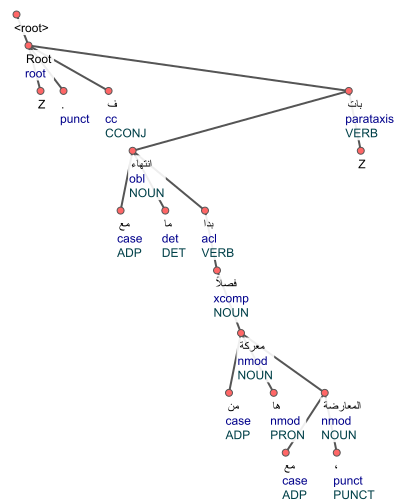
\includegraphics[scale=0.7]{img/siblingAttach-ar-1.png}
    \caption{Original Annotation}
    \label{fig:siblingAttach-ar-1}
    \end{subfigure}
    \newline
    \begin{subfigure}{\textwidth}
    \centering
    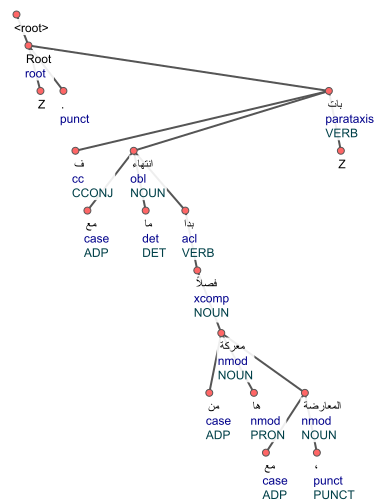
\includegraphics[scale=0.7]{img/siblingAttach-ar-2.png}
    \caption{Final Annotation}
    \label{fig:siblingAttach-ar-2}
    \end{subfigure}
    \caption{Introduced Conjunction Sandwich in \texttt{ar}}
    Note: Z is used as a placeholder for omitted text\\
    Note: Root is used as a placeholder for root of the tree\\
    Note: \textarabic{ف} (\textit{f}; And) should be attached to \textarabic{انتهاء} (\textit{aintiha'}; finishing) and not to \textarabic{بات} (\textit{bat}; become-\textit{Perf.}-\textit{3P})
    \label{fig:siblingAttach-ar}
\end{figure}

 In case of \verb|af|, the actual conjunct could not be discovered because of the improper annotation of the subtree. The modification as done by \textit{attachToSibling()} algorithm attached the conjunction to where the conjunct should have been. Attachment to the right conjunct in this case was not possible because (i) the change of levels in present annotation would bypass the enforced limit of one level; and (ii) the new attachment would have been non-projective in nature, and was therefore not allowed. Example \ref{examp:siblingAttachaf} and the associated dependency trees in Figure \ref{fig:siblingAttach-af} demonstrate this with a part of the actual sentence. As in previous example, \textit{Z} is used to denote the omitted part of the tree, while also showcasing the relative position of the root of the tree. The token of interest is marked in bold.
 
\begin{example}
\label{examp:siblingAttachaf}
\textbf{ }\\
\textbf{Text (\texttt{af}):} Deur bewusmakingsveldtogte \textbf{en} inderdaad as gevolg van die vennootskappe Z\\
\textbf{Lit:} Through awareness-campaigns \textbf{and} indeed as consequence of the partnerships ...\\ 
\textbf{Translated:} Through awareness campaigns \textbf{and} indeed because of the partnerships ...
\end{example}

\begin{figure}[H]
    \begin{subfigure}{.48\textwidth}
    \centering
    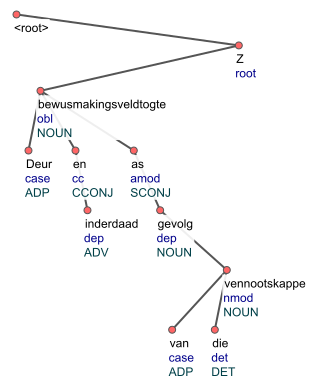
\includegraphics[scale=0.8]{img/siblingAttach-af-1.png}
    \caption{Original Annotation}
    \label{fig:siblingAttach-af-1}
    \end{subfigure}
    % \newline
    \begin{subfigure}{.5\textwidth}
    \centering
    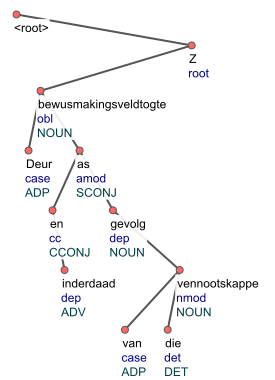
\includegraphics[scale=0.8]{img/siblingAttach-af-2.png}
    \caption{Final Annotation}
    \label{fig:siblingAttach-af-2}
    \end{subfigure}
    \caption{Introduced Conjunction Sandwich in \texttt{af}}
    \label{fig:siblingAttach-af}
    Note: Z is used as a placeholder for omitted text, and also to mark the position of the root of the tree\\
    Note: \textbf{gevolg} (consequence) should be the head of the subtree, with \textbf{as} (as) attached to it\\
    Note: \textbf{inderdaad} (indeed) should be attached to \textbf{gevolg} (consequence) after the change of subtree head\\
    Note: \textbf{en} (and) should be attached to \textbf{gevolg} (consequence) after the change of subtree head
\end{figure}

The instances of misdirected dependency in conjunctions that escaped processing by \textit{attachToSibling()} algorithm were then processed by algorithms \textit{attachToAunt()} and \textit{attachToGrandparent()} in that order. We found that the majority of these cases were still misdirected even after being processed by the overall algorithm. We discuss such cases in the next section where we discuss some insights into the processing of the algorithm step by step. Of the instances that led to a case of conjunction sandwich, the majority of the cases were caused by an annotation error, caused due to improper selection of the head of the relevant subtree. The example from \verb|af| treebank in Example \ref{examp:others-conj-sand}, and the associated dependency tree in Figure \ref{fig:others-conj-sand} demonstrates this. In the example, the conjunction sandwich is caused because of the improper annotation in the tree. The conjunction of interest is marked in bold.

\begin{example}
\label{examp:others-conj-sand}
\textbf{ }\\
\textbf{Text (\texttt{af}):} Die derde taal kan 'n amptelike \textbf{of} 'n vreemde taal wees.\\
\textbf{Lit:} The third language can a official \textbf{or} a alien language be .\\ 
\textbf{Translated:} The third language may be an official or a foreign language .
\end{example}

\begin{figure}[H]
    \begin{subfigure}{\textwidth}
    \centering
    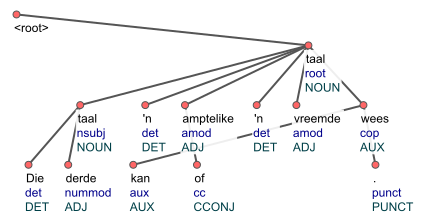
\includegraphics[scale=0.90]{img/others-conj-sand-1.png}
    \caption{Original Annotation}
    \label{fig:others-conj-sand-1}
    \end{subfigure}
    \begin{subfigure}{\textwidth}
    \centering
    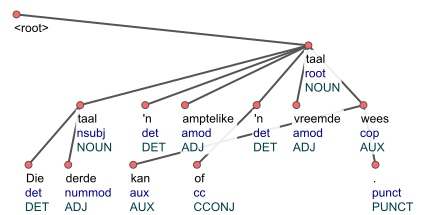
\includegraphics[scale=0.90]{img/others-conj-sand-2.png}
    \caption{Modified Annotation}
    \label{fig:others-conj-sand-2}
    \end{subfigure}
    \caption{Change in Annotation for Example \ref{examp:others-conj-sand}}
    Note: \textbf{of} (and) should be attached to \textbf{vreemde} (alien) and not to \textbf{'n} (a)\\
    \label{fig:others-conj-sand}
\end{figure}

\subsubsection{Unaffected Nodes}

By unaffected nodes, we refer to the instances of misdirected dependency which were not at all touched by the entire algorithm. We hypothesized earlier that if the rehanging of the node requires a change in more than one level (of the level of wrong conjunct), it is likely to be an annotation error that needs manual correction. We found that to be true for more than 50\% of the cases in either treebank with respect to all the unaffected cases. For the remaining cases, the major reason why the node could not be rehung was associated with the limit of deprels in \textit{attachToSibling()} algorithm. Since that was also the case for a majority of cases where the misdirected dependency persisted, we discuss the unaffected nodes with them in the final discussion.

\section{Discussion and Conclusion}

We started by identifying the cases of conjunctions that were attached non-projectively to the parent, and employed algorithms \textit{nextConjHead()} and \textit{projTempFix()} to find a better candidate. We got mixed results in all analyzed cases in both treebanks. From our understanding of the patterns exhibited in the two languages, the first algorithm works only if there exists an explicitly marked conjunct. This was true in case of \verb|af| where the conjuncts are explicitly marked with \verb|conj| deprel, but when the conjuncts are not explicitly marked (as in case of \verb|ar|), the algorithm doesn't work as intended. 

The force projectivisation in \textit{projTempFix()} algorithm did not have the desired effect. In the analysis of the instances, we found that this was mainly due to falsely annotated non-projectivities. In general, if the conjunction was in gap of another non-projective attachment to the same parent, the algorithm didn't work. The inefficiency of the algorithm in such cases could be exhibited in the form of node not being affected at all, or the new attachment eventually leading to a case of conjunction sandwich. If the conjunction (and any punctuation nodes attached to this token) is the only non-projective attachment to the parent, the algorithm would be able to make the correction effectively, and without an error.

Given the aforementioned concerns about the algorithms, it would be recommended to not use the algorithms in case of a language that displays high amount of non-projectivity in sentence structures (for example, \verb|grc|) and/or on a treebank has not been checked for the annotation consistency of the non-projective structures (as in the scope of the current experiment). Furthermore, in a case where the algorithms are used, it would be advised to have an annotator look at the corrections for higher reliability.

The common part of the pipeline started with \textit{attachToSibling()} algorithm that seeks to associate a misdirected conjunction to a sibling token, attached to the same parent. The number of cases that were found to introduce a case of conjunction sandwich could have been caused due to multiple reasons. We limited the search of a candidate head by the candidate's UPOS (more specifically, blacklisting a few UPOS) in case of a single available candidate, as mentioned earlier in the definition of the algorithm. In the event of the candidate being marked by the blacklisted UPOS, no matter the choice of deprels (except \verb|conj|), the candidate was discarded from consideration. In the algorithm, we looked for the candidate sibling within the same subtree, and not at the same level in the next subtree. This was the reason why some of the conjuncts that were located in the following subtree were discarded by the algorithm, and rather their parent (the conjunction's aunt node) was selected as the new candidate, thus introducing conjunction sandwich. The third and the final cause of conjunction sandwiches was rooted in our assumption. In the search for a candidate head, the choice was limited by the current level of attachment. We looked for a candidate at the same or at a higher level of the current attachment, thereby missing a few cases when the candidate was located at a lower level.

While the aforementioned reasons did bring about the cases of a conjunction sandwich, a relaxation of the choice of UPOS, deprels would have catastrophic effects whereby the conjunction would be rehanged to any available node. The search for a candidate at the same level, but in the following subtree is a promising approach, but it does warrant caution in the case of the suitable candidate being the aunt, and not the new candidate thus discovered. This selection of the candidate head would be non-deterministic in nature, and also depends on the annotation consistency of the given tree. Since the number of cases that were ignored, or generated conjunction sandwich into the annotation were significantly low, the problem of descending down a level to search for a candidate node can be safely ignored. In experiments where the approach was tried, the selection of the candidate node became non-deterministic, and generated a lot of false positives and introduced plethora of conjunction sandwiches.

In the evaluation, \textit{attachToSibling()} algorithms performs very well, even after accounting for sampling error. For the instances that are not processed by the algorithm, \textit{attachToAunt()} and \textit{attachToGrandparent()} algorithms don't perform as well. Upon analysis of instances that are passed to the latter algorithms, we observe a pattern. In general, if a conjunction occurs at a position such that it can change the level at which it is associated with, it will further be processed by the algorithms \textit{attachToAunt()} and \textit{attachToGrandparent()}, or would remain a case of misdirected dependency. The position of an instance in a dependency tree can be more often than not given by Equation \ref{eqn:movement-position}, where $co$ is the conjunction of interest in dependency tree $T$, attached to the node $u$.

\begin{equation}
\boxed{
    co: u \rightarrow co \And \not\exists(x) [u \rightarrow x \And co \neq x] \hspace{5mm} co, u \in T
}
\label{eqn:movement-position}
\end{equation}

A conjunction that satisfies above property can move around the tree, and can be associated to an aunt, to a grandparent, or the root of the tree, as relevant. In case the token does not satisfy the above property, and also is not affected by \textit{attachToSibling()} algorithm, it will continue being a misdirected dependency. Table \ref{tab:misdirected-before-after} shows the total number of instances with misdirected dependency, before and after the pipeline.

\begin{table}[H]
    \centering
    \begin{tabular}{|l|l|l|l|}
    \hline
    \textbf{Lang.} & \textbf{Total} & Before (in \%) & After (in \%)\\
    \hline
    \texttt{af} & 1832 & 1829 (99.84) & 106 (5.79)\\
    \texttt{ar} & 13855 & 1411 (10.18) & 398 (2.87)\\
    \hline
    \end{tabular}
    \caption{Misdirected Dependencies: Before and After}
    Note: \% is calculated against the total number of conjunctions, in the second column
    \label{tab:misdirected-before-after}
\end{table}

The algorithm \textit{attachToGrandparent()} processes more instances than \textit{attachToAunt()} algorithm, as evident from Table \ref{tab:affectedNodesOverall}. however, this processing is without any observable effect. A major reason for this is that the algorithm does not seek to find a conjunct in the grandparent's sibling, and thus just changes the level of attachment without changing the direction explicitly. This is helpful only in very limited number of cases as shown in Example \ref{examp:granny} earlier. 

The number of false positives and true positives is quite low for the joint evaluation of \textit{attachToAunt()} and \textit{attachToGrandparent()} algorithms. This prevents discussion of the efficiency of algorithms, as most of the instances that were passed on to these algorithms had no choice of candidates to attach themselves to. 

In conclusion, even though the individual algorithms of the entire pipeline vary in their results and efficiency, the approach is promising. We analysed the cases where the automation can go wrong, and the factors that would prevent automation in certain cases, and in certain language typologies.

\newpage